% Latex template: mahmoud.s.fahmy@students.kasralainy.edu.eg
% For more details: https://www.sharelatex.com/learn/Beamer

\documentclass[aspectratio=1610]{beamer}					% Document class

\setbeamertemplate{footline}[text line]{%
  \parbox{\linewidth}{\vspace*{-8pt}Semi-automated mRNA counting in single cells \hfill\insertshortauthor\hfill\insertpagenumber}}
\setbeamertemplate{navigation symbols}{}

\usepackage[english]{babel}				% Set language
\usepackage[utf8x]{inputenc}			% Set encoding

\mode<presentation>						% Set options
{
  \usetheme{default}					% Set theme
  \usecolortheme{default} 				% Set colors
  \usefonttheme{default}  				% Set font theme
  \setbeamertemplate{caption}[numbered]	% Set caption to be numbered
}

% Uncomment this to have the outline at the beginning of each section highlighted.
%\AtBeginSection[]
%{
%  \begin{frame}{Outline}
%    \tableofcontents[currentsection]
%  \end{frame}
\usepackage{graphicx}					% For including figures
\usepackage{booktabs}					% For table rules
\usepackage{hyperref}	
\usepackage{tikz-network}				% For cross-referencing
\usepackage[absolute,overlay]{textpos}
\usepackage{bm}
\usepackage[font=small,labelfont=bf]{caption}				% For cross-referencing

\title{Interferon-$\gamma$ induction of GBP5 expression in HeLa cells}	% Presentation title
\author{Clayton W. Seitz}								% Presentation author
\date{\today}									% Today's date	

\begin{document}

% Title page
% This page includes the informations defined earlier including title, author/s, affiliation/s and the date
\begin{frame}
  \titlepage
\end{frame}


% The following is the most frequently used slide types in beamer
% The slide structure is as follows:
%
%\begin{frame}{<slide-title>}
%	<content>
%\end{frame}

\begingroup
\setbeamertemplate{footline}{}
\begin{frame}{Single-cell RNA-seq identifies GBP5 as a memorized gene}
\begin{figure}
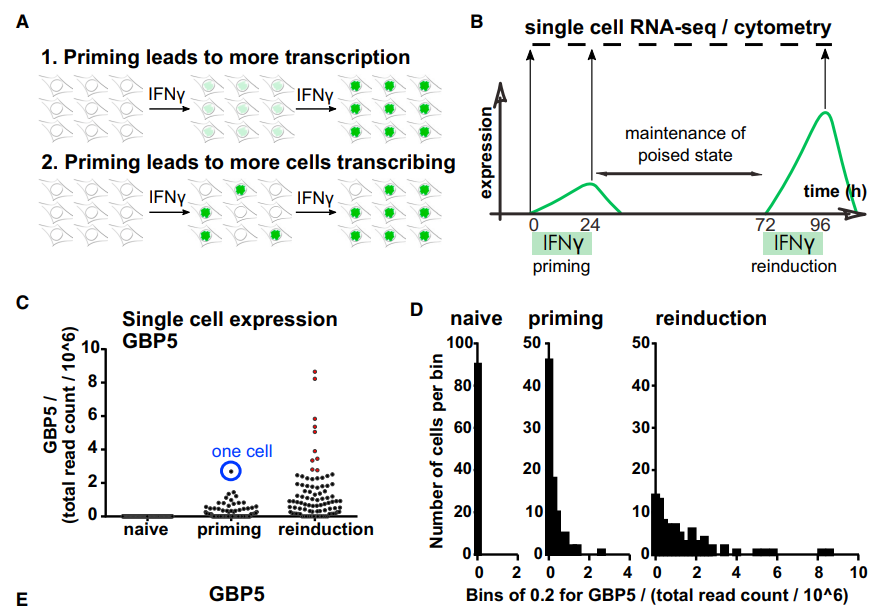
\includegraphics[width=11cm]{figure-3.png}
\end{figure}
Siwek et al. \textit{Activation of Clustered IFNg Target Genes...}. Molecular Cell 2020
\end{frame}
\endgroup

\begin{frame}{GBP5 imaging approach}
High-throughput 3D acquisition of DAPI + FISH probes for GAPDH, GBP5 mRNA in Hela cells on \#1.5 chambered coverglass, 60x oil
\begin{center}
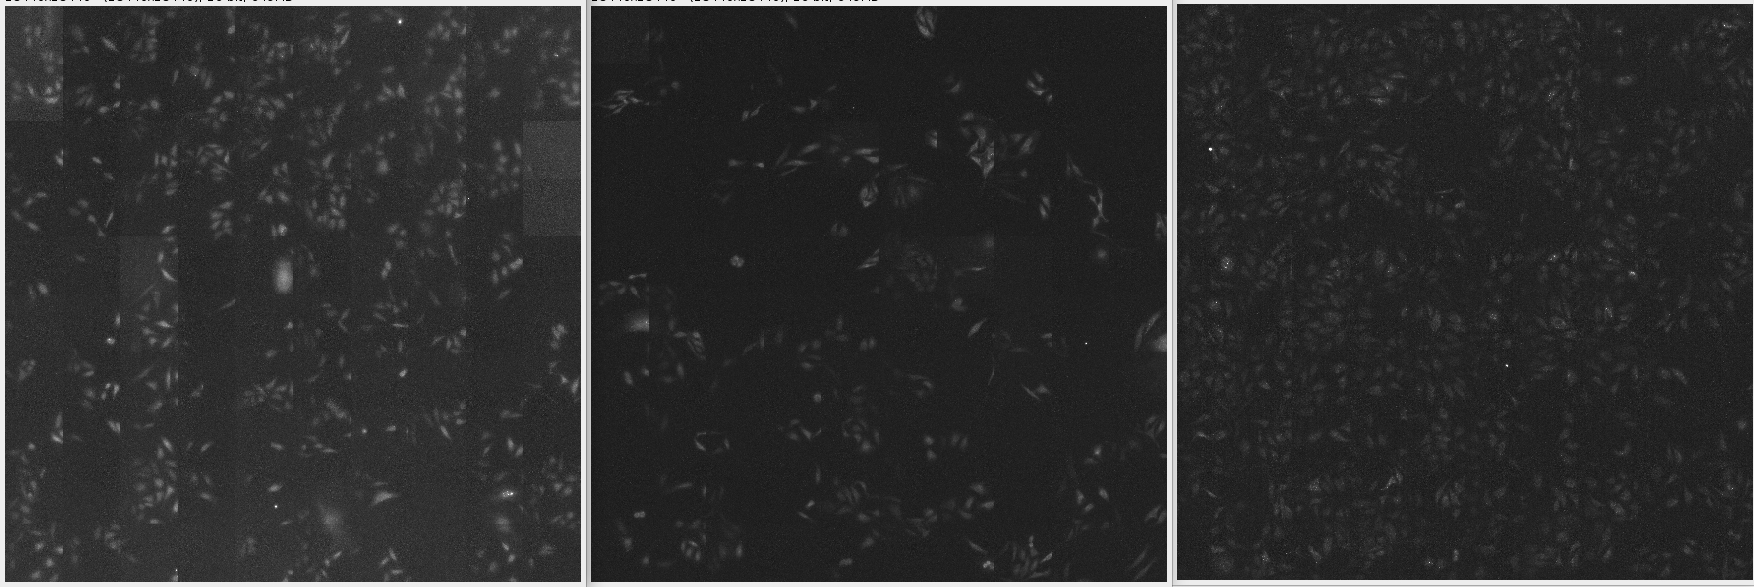
\includegraphics[width=1.0\textwidth]{Tiles.png}
\end{center}
But as usual, segmentation is the rate-limiting step
\end{frame}

\begin{frame}{Training a semantic segmentation with cross-entropy loss (log loss)}
\vspace{0.1in}
100 256\;x\;256 images (downsampled GAPDH channel), 80 train + 20 validation, 

\begin{center}
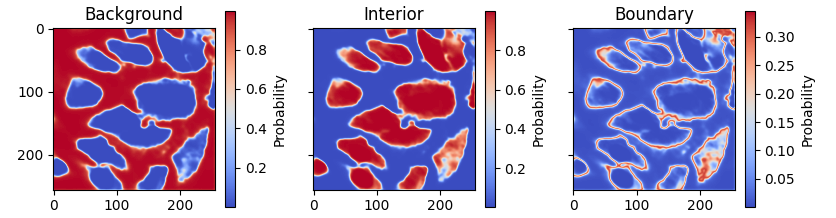
\includegraphics[width=1\textwidth]{Softmax.png}
\end{center}

We train a 3-class semantic segmentation model with cross-entropy loss:

\begin{equation*}
\mathcal{L} = \sum_{i,j} \log p_{ij}(\tilde{x}) = \sum_{i,j} \log \frac{\exp(-s_{ij}(\tilde{x}))}{\sum_{x\in\chi} \exp(-s_{ij}(\tilde{x}))}
\end{equation*}

$p_{ij}$ is the probability the model assigns a pixel to the true class $\tilde{x} \in \{\textrm{a}, \textrm{b}, \textrm{c}\}$

\end{frame}


\end{document}